%%% $Id$
%%% Copyright (C) 2002 Greg J. Badros <greg.badros@infospace.com>
%%
%
% This file should be compiled with V1.0 of "www2003-submission.cls"
%
% ----------------------------------------------------------------------------------------------------------------
% This .tex file (and associated .cls V1.0) produces:
%       1) NO Permission Statement
%       2) WWW'03-specific conference (location) information
%       3) The Copyright Line with ACM data
%       4) NO page numbers
%
% ---------------------------------------------------------------------------------------------------------------
% This .tex source is an example which *does* use
% the .bib file (from which the .bbl file % is produced).
% REMEMBER HOWEVER: After having produced the .bbl file,
% and prior to final submission, you *NEED* to 'insert'
% your .bbl file into your source .tex file so as to provide
% ONE 'self-contained' source file.
%

\documentclass{www2003-submission}
\usepackage{times}
\usepackage{moreverb}
\usepackage{floatflt}
\usepackage{url}

\newcommand{\B}{\discretionary{}{}{}}
\newcommand{\smtt}{\small}
\newcommand{\smtexttt}[1]{{\small\texttt{#1}}}
\newcommand{\figref}[1]{Fig.~\ref{fig-#1}}
\newcommand{\tableref}[1]{Table~\ref{#1}}
\newcommand{\tm}{{\scriptsize $^{\mbox{tm}}$}}

\begin{document}
%
\title{The Extensible Templating Language: \\
       Improving Analysis of Markup Generating Code}

\numberofauthors{1}

\author{
%
% The command \alignauthor (no curly braces needed) should
% precede each author name, affiliation/snail-mail address and
% e-mail address. Additionally, tag each line of
% affiliation/address with \affaddr, and tag the
%% e-mail address with \email.
\alignauthor Greg J. Badros\\
       \affaddr{InfoSpace, Inc., 601 108th Ave. NE, Suite 1200, Bellevue, WA 98004, USA}\\
       \email{greg.badros@infospace.com}
}
\date{2 November 2002}
\maketitle
\begin{abstract}
ETL....
\end{abstract}

% A category with only the three required fields
%% GREGB:FIXME::
\category{D.2}{Software}{Software Engineering}
\category{D.3}{Software}{Programming Languages}

% GREGB:FIXME:: any terms?
%\terms{}

\keywords{Static analysis, web server, templates, XML, XSLT, markup, WML, HTML.}

\section{Introduction}

Server-side dynamically-generated web pages have become increasingly
common and more complex.  The loosely-coupled client/\B{}server model
implied by the current breed of applications deployed via the World
Wide Web presents substantial new complexities for application
developers, and a variety of new programming languages and paradigms
attempt to address these novel problems.  One important characteristic
of this new world of software development is the need to generate HTML
or other markup languages to describe the client-side presentation and
behaviour.

The original server-side dynamic markup-generation capabilities of the
Web were defined by CGIs.\cite{CGI} For each request, the web server
maps HTTP request details into environment variables, command-line
arguments, and the standard file descriptors.  In particular, the
standard output written by that process was sent by the Web server as
the response to the client browser (instead of simply responding with
an unchanging file from disk).  Over time, various techniques arose to
reduce the cost of each request: extension mechanisms such as the
Apache module system~\cite{ApacheModules} and scripting languages
hosted by the Web server have increased performance by eliminating
process creation overhead.

The variety of server-side scripting is dominated by expressive and
flexible general-purpose programming languages such as
Java~\cite{Java}, Perl~\cite{Perl}, and PHP~\cite{PHP}.  Ironically,
the languages are then used in fairly restricted ways, often being
tied to a templating language (e.g., JSP~\cite{JSP} for Java or
HTML::Template~\cite{HTML-Template} for Perl).  For example, consider
the PHP template in \figref{php-books}.  The only constructs required
by the template are a) some means of populating a data model from the
back-end business logic (line 1); b) data-driven iteration (line
5-6); and c) simple expression evaluation to access parts of the data
model (lines 7 and 9). % GREGB:FIXME:: check these line numbers

\begin{figure}[htbp]
\begin{listing}{1}
<? $books = GetBooks(...); ?>
<html>
 <table>
  <? for ($i = 0; 
           $i < count($books); ++$i) { ?>
   <tr>
     <td><? print($books[$i][author]); ?>
         </td>
     <td><? print($books[$i][title]); ?>
         </td>
   </tr>
  <? } ?>
 </table>
</htm>
\end{listing}%$
\caption{PHP template illustrating the simplicity of the programming
language constructs required by typical templates.
\label{fig-php-books}}
\end{figure}

Unfortunately, for most contemporary web application development
frameworks, the restrictions desired of the front-end templating layer
are imposed only by process and convention.  Template authors are
asked to limit themselves to a subset of the available features of a
language as a means of facilitating scalable, secure, well-behaved
systems.  Importantly, however, there is nothing inherent that
prevents template executions from, for example, making individual
database connections (which would impact performance) or maintaining
undesirable server-side state (which would impose additional
requirements on the load-balancing mechanism and reduce scalability).
These concerns are intensified because many development organizations
encourage a strong separation between the web developers and back-end
application developers. While web developers have substantial
expertise in HTML, user-interface design, and client-side scripting,
their responsibilities often do not include consideration of the
larger architecture.

Another substantial problem with existing templating technologies is
that they often involve the lexical mixing of two separate programming
paradigms.  JSP, for example, is implemented in terms of a
pre-processing rewrite of the template into a Java servlet.~\cite{JaveServlet}
Pre-processing approaches are convenient for programmer expressiveness
but have a huge hidden cost in complicating software engineering
analyses and tools that would otherwise help understand, maintain, and
evolve the complex systems~\cite{PCP3,EvilMacros,StroustropDnEChapterAboutCpp}.
The precise analysis of an arbitrary JSP template necessarily requires
full knowledge of both the rewrite rules and the semantics of Java.

%% GIVE EXAMPLES OF VALUABLE ANALYSES!!!
\subsection{Analysis of markup templates}

The various templating languages all have one primary goal: to
generate markup to be returned to the requesting user agent.  It is
important that the markup created conforms to appropriate Internet
standards.  For example, WML markup needs to first be well-formed XML
and second be valid with respect to the appropriate
schemata~\cite{WML}.  Although HTML browsers are more forgiving of
improper syntax, best-practices still dictate that the markup returned
be in compliance with the HTML specification~\cite{HTML}.  
Popular templating languages including PHP, JSP, ASP, and others
all process arbitrary text and are ignorant of the rules of the markup
being generated: the mistaken close tag on line 14 of \figref{php-books}
goes unnoticed by PHP.

Tools such as HTMLTidy~\cite{HTMLTidy} are available to check the
responses from servers for conformance, but often testing involves
simply using various browsers to exercise the application while
looking for bugs.  Both of these approaches require exhaustively
visiting every page of interest--often a very large search space.
Ideally, we would prefer a way to analyze the source templates
themselves to gain confidence that they will, in fact, generate proper
markup.  If static analysis of templates can rule out the possibility
of certain kinds of errors, testing time and costs can be dramatically
reduced.

Another important requirement is to support ad-hoc queries of
the source code templates. For small and simple dynamic web applications,
the automated analysis of templates is often unnecessary: a web
developer or two understands all of the code.  Over time, however,
these simple applications easily grow in size and complexity such that
tools analyzing the templates become an essential part of maintaining
and evolving the system. For example, a site may wish to add an extra
input field to all of its registration forms.  If a generic form is
not already factored out into a common location, the first step in
approaching the task is finding all of the registration forms.  Or
suppose a new handheld device has a bug in handling an HTTP response
header: we need to identify all the code in the system that may
generate that header.

Typically, web developers approach to above scenarios with an arsenal
of imprecise lexical tools such as \smtexttt{find} and
\smtexttt{grep}.  While searching for a substring or regular
expression may satisfy some simple queries, when the desired query has
additional structure, lexical approaches fall short.  No regular
expression will let us identify all unreachable templates (i.e., we
want to find dead code) so that we can simplify the application by
eliminating those templates.  To analyze more deeply, we need to
uncover the structure of the templating language.  Typically, that
requires a language-specific parsing approach for which fewer tools
exist.

\subsection{XML supports analyses}

An increasingly popular approach to performing structured queries of
programming language source code is to use standard XML tools such as
XSLT~\cite{XSLT} and XQuery~\cite{XQuery} to operate over a
complementary XML-based representation~\cite{JavaML,others}.  With a
carefully-chosen XML representation, valuable semantics of the code
are immediately available to XPath expressions, thus facilitating a
broad class of source code tools.  However, for a general-purpose
programming language, XML is unwieldy for use as the primary
representation: the conventional grammer-based language is edited by
humans and is only converted into XML for the tools to leverage.

This research applies the benefits of an XML representation of source
code to domain-specific markup templating languages.  Importantly,
web developers working with templating languages are already writing
markup directly, thus making it natural for them to express the logic
of their dynamic templates directly in markup as well.  This
observation eliminates the dual representation problem that limits the
value of XML when applied to general purpose programming language.

In this paper, I introduce the Extensible Templating Language.  From
one perspective, ETL is a 100\% XML-based templating language that
embeds programming language constructs directly in the XML
representation, intermingled with literal target-language markup.
Alternatively, we can view ETL as an imperative domain-specific
programming language that uses XML as its surface syntax and
simplifies the writing of programs that generate markup languages.

ETL leverages the well-formedness and local-validity checks of the
source template to support the correctness of the generated response
markup.  Additionally, because of its use of XML as a representation,
it simplifies ad-hoc software engineering analyses to better support
evolution and maintenance of large dynamic web applications.  We have
built an ETL runtime inside of a production-quality web server, the
Extensible Templating Language Server.  ETLS is currently employed by
InfoSpace to serve over forty million requests per day using over
sixty thousand ETL templates.

\subsection{Outline of paper}

Section \ref{sec-} ....

%%% 
%\section{Background}

%% JSP/XML
%% XSLT

%\subsection{Current templating strategies}

%\subsection{Comparison of approaches}

%\begin{table}
%\centering
%\caption{Summary of existing templating approaches.}
%\begin{tabular}{|c|c|l|} \hline
%\\ \hline
%\hline\end{tabular}
%\end{table}


%%% 
\section{Extensible Templating Language}


*** increase the probability that a program that checks does the right thing

*** reduce development cycle time, greatly reduce testing costs

*** approximate analyses should be easy, precise analyses should be possible
    (e.g., finding all the variables used by a template)


\begin{figure}[htbp]
\begin{listing}{1}
<?xml version="1.0"?>
<bl:template xmlns:bl="http://www....">
 <bl:set var="#xml/books">...</bl:set>
 <html>
  <table>
   <bl:for-each var="#xml/books/book">
    <tr> 
     <td><bl:get var="@author"/></td>
     <td><bl:get var="@title"/></td>
    </tr>
   </bl:for-each>
  </table>
 </html>
</bl:template>
\end{listing}%$
\caption{The ETL template corresponding to \figref{php-books}'s PHP
code. Because ETL is required to be well-formed XML, the developer
avoids the mistake from line 14 of the PHP example.
\label{fig-etl-books}}
\end{figure}

\subsection{Primitives}

\subsection{Variables \& slots}

\subsection{Reserved variables}

\subsection{Buckets}

\subsection{Cobrand profiles}

\subsection{Template selection}

% bl:call, argument passing

\subsection{Transformers \& formatters}

\subsection{Comments}

\subsection{Controlling whitespace}

Whitespace characters\footnote{Whitespace that is not a part of the
XML Infoset~\cite{XML-infoset}, such as whitespace between attrbutes inside element
tags, is managed via XML processing rules and is not controlled by the
rules described in this section.} in a source template have mixed uses.  In some
cases, the developer wishes to improve the readability of the program
by using indentation or blank lines.  In other cases, the whitespace
is intended to be copied into the output document or a variable's
value.  The \smtexttt{xml:space} attribute provided by the XML
standard~\cite[2.10]{XML} is not sufficiently expressive to support
the various needs of the template author.

\begin{figure}[bt]
\begin{centering}
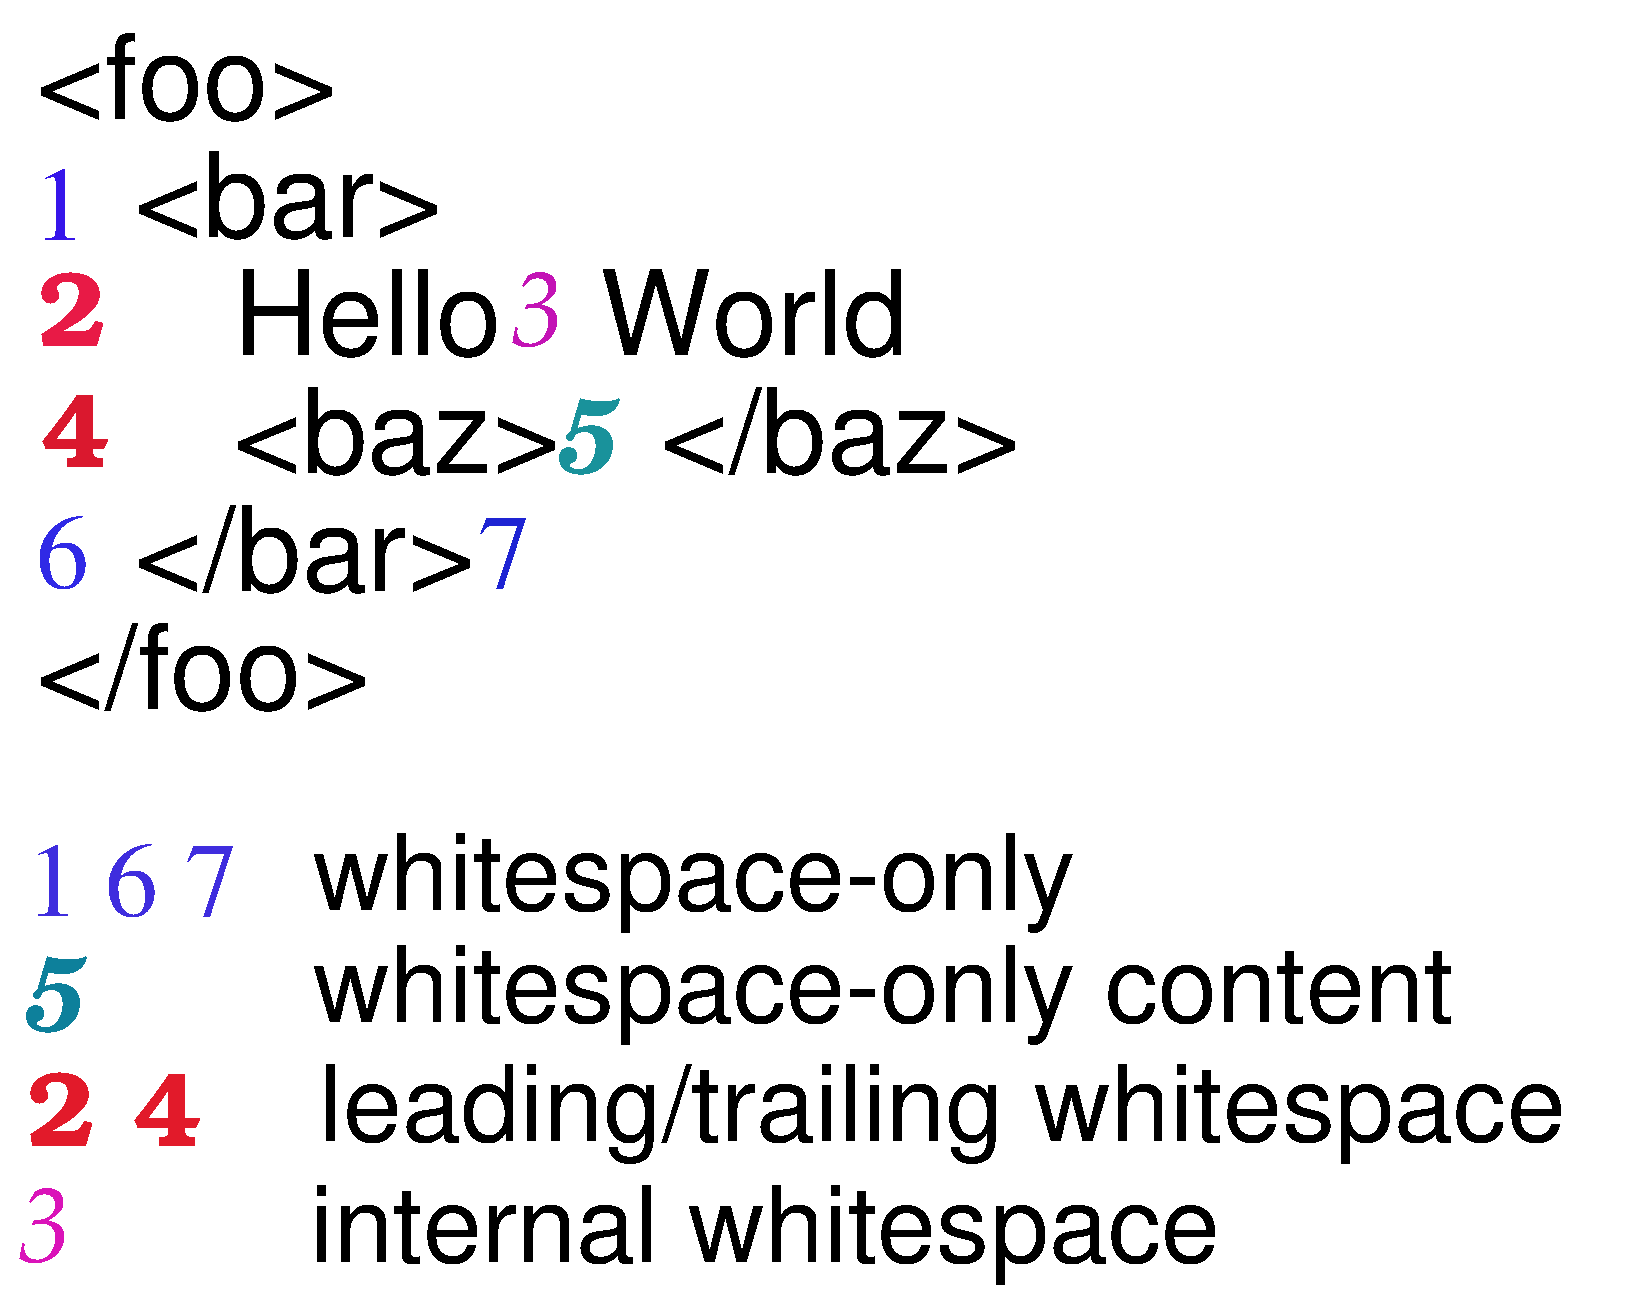
\includegraphics[height=1.5in]{etl-whitespace-rules.eps}
\caption{The various classes of whitespace nodes in XML. \label{fig-ws-rules}}
\end{centering}
\end{figure}

ETL permits fine-grained control over the whitespace that will be
generated via two orthogonal special attributes that are allowed on
every XML element in source ETL documents: \smtexttt{@bl:space-nodes}
and \smtexttt{@bl:text-nodes}.  These attributes are inherited by
contained (i.e., children) elements and their contents unless
overridden.  They control the various classes of whitespace
illustrated in \figref{ws-rules} as follows.

\begin{itemize}
\item \smtexttt{@bl:space-nodes} controls whitespace-only (and
      whitespace-only content) nodes (1, 5, 6, and 7 in the figure).
\item \smtexttt{@bl:text-nodes} controls leading/internal/trailing whitespace of
      text nodes (2, 3, and 4 in the figure).
\end{itemize}

The allowed settings for \smtexttt{@bl:space-nodes} are:

\begin{description}
  
\item[\smtexttt{preserve}] Leave the whitespace unchanged
      
\item[\smtexttt{compact}] Replace sequences of 1 or more
      whitespace characters with a single space (0x20)
      
\item[\smtexttt{strip}] Eliminate the whitespace entirely

\item[\smtexttt{normalize}] Strip whitespace nodes that contain only
newline (0x0A) characters entirely; replace sequences of 1 or more
whitespace characters that include a space or a tab with a single
space (0x20)

\end{description}

In addition to the above, \smtexttt{@bl:text-nodes} permits assymetric
handling of the left and right sides of the text nodes via values
\smtexttt{compact-(left|right)} and \smtexttt{trim-(left|right)}. 
Importantly, all of these whitespace rules are statically-scoped:
a called template does not inherit the attributes from the calling
templates attribute annotations.

\subsection{Literal markup}

% conditional tags
% at:*
% ?foo syntax
% building URIs

\subsection{Control constructs}

\subsection{Custom tags}

\subsection{Invoking applications}


%%% 
\section{Benefits of ETL}

ETL has an integrated development environment that was very
easy to build by leveraging the XSD schema that defines the language
(\figref{homesite-screenshot}).

** development environment completion
** validation for deep checking before deployment
** analysis 
** pretty-printing 
** source->source transformation 
** new abstractions 
** reduce app-level security holes (ref. scott \& sharp)


\begin{figure}[tb]
\begin{centering}
\hspace*{-0.05\linewidth}\includegraphics[width=1.1\linewidth]{homesite-screenshot.eps}
\caption{A screenshot of the integrated development environment based
on Homesite.  By using custom tag information generated automatically
from the XSD schema for ETL, the environment supports automatic
completion of names of elements and their valid attributes.  Help
information extracted from the server codebase is also readily
available in the IDE\@.
\label{fig-homesite-screenshot}}
\end{centering}
\end{figure}


%%% 
\section{Implementation \& experience}

** ETLS, its goals, backward-compatibility needs

** Server principles
*** be an appliance box: everything via HTTP
*** support MS management interfaces (mmc, win* service)

ETL has a debugger (\figref{debugger-screenshot}).  Solve fundamental
problem of needing to have stderr output for web development.

% ?etl-* parameters
% security
% inspadmin:* directives & the startup configuration file

\begin{figure}[tb]
\begin{centering}
\hspace*{-0.07\linewidth}\includegraphics[width=1.15\linewidth]{debugger-screenshot.eps}
\caption{A screenshot of the debugger.
\label{fig-debugger-screenshot}}
\end{centering}
\end{figure}


\begin{figure}[tb]
\begin{centering}
\hspace*{-0.05\linewidth}\includegraphics[width=1.1\linewidth]{etls-admin.eps}
\caption{The ETL Server's administration pages.
\label{fig-etls-admin}}
\end{centering}
\end{figure}



\begin{figure}[htbp]
\begin{verbatim}
Template `books.html.etl' has 0 errors.
0 template('books.html.etl') {
1  set_simple(#xml/books := '...')
2  #nocmd('<html>','</html>') {
3   #nocmd('<table>','</table>') {
4    for-each(#xml/books/book) {
5     #nocmd('<tr>','</tr>') {
6      #nocmd('<td>','</td>') {
7       get(@author)
       } // #nocmd('<td>','</td>')
8      #nocmd('<td>','</td>') {
9       get(@title)
       } // #nocmd('<td>','</td>')
      } // #nocmd('<tr>','</tr>')
     } // for-each(#xml/books 'book')
    } // #nocmd('<table>','</table>')
   } // #nocmd('<html>','</html>')
  } // template('books.html.etl')
\end{verbatim}%$
\caption{A server-generated decompilation of the internal representation
of the ETL template from \figref{etl-books}.  The nesting of elements
is preserved, but the byte-codes have been linearized for performance.
\label{fig-etl-decompile}}
\end{figure}


%%% 
\section{Related work}

%% LAML
%% BigWig


%%% 
\section{Conclusions \& future work}

* Restate contribution, stress in use


** XML infoset and non-infoset artifacts
*** a bit problematic for source->source and for representing literal markup
** alternate syntax (a la stylescript) for other purposes
*** importantly, has an implied XML data model (e.g., can be algorithmically turned into the other syntax)
** math and conditionals
** generalized content-slot
** improvements to XSD to enable better validation
*** e.g., either/or attributes for slots
*** custom tag element definitions
** levels of strictness
** data flow analyses to infer needs for xmlencoding of variable values
** taint tracking of input variables
** better warning/error reporting in terms of the pre-macro-transformed source template


%ACKNOWLEDGMENTS are optional
\section{Acknowledgments}
This research is supported by InfoSpace and its advanced server
development group.  I thank Russ Arun and Steve Newman for their early
recognition of the value of this approach and their support.  ETL
itself was designed in collaboration with Abhishek Parmar and is
influenced by the legacy language of its predecessor web server which
was implemented by Jean-Remy Facq.  The ETL Server system was built by
the author along with Abhishek Parmar, Venkatesh Juryala, Sridhar
Koneru, Mark Sandori, Michael Harrison, Kris Bradley, Sunil Thomas,
Angela Plyler, and Howard Zhao.  Testing of ETLS was ably performed by
Zine Rif, Sriram Krishnan, Michael Schaffer, Shavkat Azimov, Jeff
Wells, Ilian Georgeiw, and Russell Ashmun, and credit goes to Antonio
Casacuberta for continued support of the server group.  I also thank
Jeff Torgerson, Matthew Benedict, and Vasanth Cattamanchi for their
contributions to the system. ETLS is a trademark of InfoSpace, Inc.


\bibliographystyle{abbrv}
\bibliography{etl-www2003}  % sigproc.bib is the name of the Bibliography in this case

%
%\balancecolumns
\appendix
%Appendix A
%\section{}
%\balancecolumns % GM July 2000

\end{document}
